% supplementary_material_sixsphere.tex
%
% What a Cusp Rolls Up, and What Cannot Be Rolled Up.
% Every number below is a macro written by paper/make_sixsphere_facts.py,
% which recomputes it from pyCICY.sixsphere_search; the fallbacks in the
% preamble typeset as "?" if the facts have not been generated.
%
%   python3 paper/make_sixsphere_facts.py      (about two minutes)
%   make sixsphere-paper

\documentclass[11pt,a4paper]{article}

\usepackage[T1]{fontenc}
\usepackage[utf8]{inputenc}
\usepackage[margin=1in]{geometry}
\usepackage[protrusion=true,expansion=false]{microtype}
\usepackage{amsmath,amssymb,amsthm}
\usepackage{graphicx}
\usepackage{booktabs}
\usepackage{enumitem}
\usepackage{xcolor}
\usepackage[hidelinks]{hyperref}
\usepackage[nameinlink,capitalize]{cleveref}
\IfFileExists{orcidlink.sty}{\usepackage{orcidlink}}%
  {\newcommand{\orcidlink}[1]{}}

\graphicspath{{figures/}}

% Numbers computed by paper/make_sixsphere_facts.py. Defined here as a
% fallback so the document still typesets if the facts have not been
% generated yet; the \input below overrides them with the real values.
\newcommand{\SSSurveyPairs}{?}\newcommand{\SSSurveyPairsWord}{?}
\newcommand{\SSNoCuspCount}{?}\newcommand{\SSStarCuspCount}{?}
\newcommand{\SSMinPThreeSix}{?}\newcommand{\SSMinPFourSix}{?}
\newcommand{\SSCuspNThreeSix}{?}
\newcommand{\SSSurveyTable}{? & ? & ? & ? & ? \\}
\newcommand{\SSBox}{?}\newcommand{\SSTried}{?}\newcommand{\SSOrders}{?}
\newcommand{\SSCusp}{?}\newcommand{\SSCoinv}{?}\newcommand{\SSClosure}{?}
\newcommand{\SSUnimod}{?}\newcommand{\SSMOneChoices}{?}
\newcommand{\SSStabBoxes}{?}\newcommand{\SSStabBoxMin}{?}
\newcommand{\SSStabBoxMax}{?}\newcommand{\SSStabFinal}{?}
\newcommand{\SSStabCusp}{?}
\newcommand{\SSClasses}{?}\newcommand{\SSClassesWord}{?}
\newcommand{\SSClassSize}{?}\newcommand{\SSGoodInvariant}{?}
\newcommand{\SSOtherInvariants}{?}\newcommand{\SSNearMissMins}{?}
\newcommand{\SSPaperConj}{?}\newcommand{\SSPaperConjDet}{?}
\newcommand{\SSRepOne}{?}\newcommand{\SSRepTwo}{?}
\newcommand{\SSLavesSites}{?}\newcommand{\SSLavesBonds}{?}
\newcommand{\SSLavesIncidences}{?}\newcommand{\SSSpectreSites}{?}
\newcommand{\SSSpectreVertexValence}{?}\newcommand{\SSNearHatSites}{?}
\newcommand{\SSWComponents}{?}\newcommand{\SSWCurves}{?}
\newcommand{\SSWPoints}{?}\newcommand{\SSEW}{?}
\newcommand{\SSMirrorConj}{?}\newcommand{\SSMirrorDet}{?}
\newcommand{\SSDetQZero}{?}\newcommand{\SSDualDetForm}{?}
\newcommand{\SSClassesPeriods}{?}\newcommand{\SSClassesSpectre}{?}
\newcommand{\SSShareGeometry}{?}\newcommand{\SSShareLatticeSpectre}{?}
\newcommand{\SSLeanFacts}{?}\newcommand{\SSLeanChoiceFree}{?}
\newcommand{\SSLeanNew}{?}\newcommand{\SSLeanStatus}{?}
\newcommand{\SSLeanChecked}{?}
\newcommand{\SSDPVolume}{?}\newcommand{\SSDPBoundary}{?}
\newcommand{\SSDPDual}{?}\newcommand{\SSDPProduct}{?}
\newcommand{\SSDPBoundSym}{?}\newcommand{\SSDPKTwo}{?}
\newcommand{\SSDPRays}{?}
\newcommand{\SSKodairaCandidates}{?}\newcommand{\SSKodairaTotals}{?}
\newcommand{\SSKodairaTriple}{?}
\newcommand{\SSERootsEight}{?}\newcommand{\SSERootsSeven}{?}
\newcommand{\SSERootsSix}{?}\newcommand{\SSEDiscSeven}{?}
\newcommand{\SSEDiscSix}{?}\newcommand{\SSEDiscSixA}{?}
\newcommand{\SSMWRank}{?}\newcommand{\SSGuardRefused}{?}
\IfFileExists{figures/sixsphere_facts.tex}{% generated by paper/make_sixsphere_facts.py -- do not edit
% providecommand+renewcommand so this works whether or not
% the fallback definitions in the .tex have been read first
\providecommand{\SSBox}{}\renewcommand{\SSBox}{5}
\providecommand{\SSClassSize}{}\renewcommand{\SSClassSize}{8}
\providecommand{\SSClasses}{}\renewcommand{\SSClasses}{4}
\providecommand{\SSClassesPeriods}{}\renewcommand{\SSClassesPeriods}{\{-3,-1,1,3\}}
\providecommand{\SSClassesSpectre}{}\renewcommand{\SSClassesSpectre}{\{1,6,10,15\}}
\providecommand{\SSClassesWord}{}\renewcommand{\SSClassesWord}{four}
\providecommand{\SSClosure}{}\renewcommand{\SSClosure}{84}
\providecommand{\SSCoinv}{}\renewcommand{\SSCoinv}{84}
\providecommand{\SSCusp}{}\renewcommand{\SSCusp}{272}
\providecommand{\SSCuspNThreeSix}{}\renewcommand{\SSCuspNThreeSix}{2}
\providecommand{\SSDPBoundSym}{}\renewcommand{\SSDPBoundSym}{32}
\providecommand{\SSDPBoundary}{}\renewcommand{\SSDPBoundary}{6}
\providecommand{\SSDPDual}{}\renewcommand{\SSDPDual}{6}
\providecommand{\SSDPKTwo}{}\renewcommand{\SSDPKTwo}{6}
\providecommand{\SSDPProduct}{}\renewcommand{\SSDPProduct}{36}
\providecommand{\SSDPRays}{}\renewcommand{\SSDPRays}{6}
\providecommand{\SSDPVolume}{}\renewcommand{\SSDPVolume}{6}
\providecommand{\SSDetQZero}{}\renewcommand{\SSDetQZero}{36}
\providecommand{\SSDualDetForm}{}\renewcommand{\SSDualDetForm}{36s^4}
\providecommand{\SSEDiscSeven}{}\renewcommand{\SSEDiscSeven}{2}
\providecommand{\SSEDiscSix}{}\renewcommand{\SSEDiscSix}{3}
\providecommand{\SSEDiscSixA}{}\renewcommand{\SSEDiscSixA}{6}
\providecommand{\SSERootsEight}{}\renewcommand{\SSERootsEight}{240}
\providecommand{\SSERootsSeven}{}\renewcommand{\SSERootsSeven}{126}
\providecommand{\SSERootsSix}{}\renewcommand{\SSERootsSix}{72}
\providecommand{\SSEW}{}\renewcommand{\SSEW}{2}
\providecommand{\SSGoodInvariant}{}\renewcommand{\SSGoodInvariant}{\{1,5\}}
\providecommand{\SSGuardRefused}{}\renewcommand{\SSGuardRefused}{refuses}
\providecommand{\SSKodairaCandidates}{}\renewcommand{\SSKodairaCandidates}{4}
\providecommand{\SSKodairaTotals}{}\renewcommand{\SSKodairaTotals}{8, 12, 14, 18}
\providecommand{\SSKodairaTriple}{}\renewcommand{\SSKodairaTriple}{\mathrm{IV}^*+\mathrm{III}+\mathrm{I}_1}
\providecommand{\SSLavesBonds}{}\renewcommand{\SSLavesBonds}{102}
\providecommand{\SSLavesIncidences}{}\renewcommand{\SSLavesIncidences}{102}
\providecommand{\SSLavesSites}{}\renewcommand{\SSLavesSites}{61}
\providecommand{\SSLeanChecked}{}\renewcommand{\SSLeanChecked}{true}
\providecommand{\SSLeanChoiceFree}{}\renewcommand{\SSLeanChoiceFree}{29}
\providecommand{\SSLeanFacts}{}\renewcommand{\SSLeanFacts}{34}
\providecommand{\SSLeanNew}{}\renewcommand{\SSLeanNew}{4}
\providecommand{\SSLeanStatus}{}\renewcommand{\SSLeanStatus}{machine-checked by the Lean~4 kernel in this build}
\providecommand{\SSMOneChoices}{}\renewcommand{\SSMOneChoices}{2}
\providecommand{\SSMWRank}{}\renewcommand{\SSMWRank}{1}
\providecommand{\SSMinPFourSix}{}\renewcommand{\SSMinPFourSix}{2}
\providecommand{\SSMinPThreeSix}{}\renewcommand{\SSMinPThreeSix}{3}
\providecommand{\SSMirrorConj}{}\renewcommand{\SSMirrorConj}{\begin{pmatrix}1 & 6 & -6 & -2 \\ 0 & 0 & 1 & -1 \\ 0 & 1 & 0 & -1 \\ 0 & 0 & 0 & -1\end{pmatrix}}
\providecommand{\SSMirrorDet}{}\renewcommand{\SSMirrorDet}{1}
\providecommand{\SSNearHatSites}{}\renewcommand{\SSNearHatSites}{97}
\providecommand{\SSNearMissMins}{}\renewcommand{\SSNearMissMins}{6, 2, 3}
\providecommand{\SSNoCuspCount}{}\renewcommand{\SSNoCuspCount}{4}
\providecommand{\SSOrders}{}\renewcommand{\SSOrders}{49446}
\providecommand{\SSOtherInvariants}{}\renewcommand{\SSOtherInvariants}{$\{0,6\}$, $\{2,4\}$, $\{3\}$}
\providecommand{\SSPaperConj}{}\renewcommand{\SSPaperConj}{\begin{pmatrix}1 & 3 & -3 & -2 \\ 0 & 1 & 0 & 0 \\ 0 & 0 & 1 & -1 \\ 0 & 0 & 0 & -1\end{pmatrix}}
\providecommand{\SSPaperConjDet}{}\renewcommand{\SSPaperConjDet}{-1}
\providecommand{\SSRepOne}{}\renewcommand{\SSRepOne}{\begin{pmatrix}1 & -3 & 0 & -2 \\ 0 & -1 & 1 & -2 \\ 0 & -1 & 0 & 0 \\ 0 & 0 & 0 & 1\end{pmatrix}}
\providecommand{\SSRepTwo}{}\renewcommand{\SSRepTwo}{\begin{pmatrix}1 & 0 & 0 & 0 \\ 0 & 0 & -1 & 0 \\ 0 & 1 & 0 & 1 \\ 0 & 0 & 0 & 1\end{pmatrix}}
\providecommand{\SSShareGeometry}{}\renewcommand{\SSShareGeometry}{\{1,3\}}
\providecommand{\SSShareLatticeSpectre}{}\renewcommand{\SSShareLatticeSpectre}{\{1,6\}}
\providecommand{\SSSpectreSites}{}\renewcommand{\SSSpectreSites}{97}
\providecommand{\SSSpectreVertexValence}{}\renewcommand{\SSSpectreVertexValence}{1}
\providecommand{\SSStabBoxMax}{}\renewcommand{\SSStabBoxMax}{11}
\providecommand{\SSStabBoxMin}{}\renewcommand{\SSStabBoxMin}{3}
\providecommand{\SSStabBoxes}{}\renewcommand{\SSStabBoxes}{\pm3, \pm4, \pm5, \pm8, \pm11}
\providecommand{\SSStabCusp}{}\renewcommand{\SSStabCusp}{136, 200, 272, 760, 1488}
\providecommand{\SSStabFinal}{}\renewcommand{\SSStabFinal}{32, 32, 32, 32, 32}
\providecommand{\SSStarCuspCount}{}\renewcommand{\SSStarCuspCount}{2}
\providecommand{\SSSurveyPairs}{}\renewcommand{\SSSurveyPairs}{9}
\providecommand{\SSSurveyPairsWord}{}\renewcommand{\SSSurveyPairsWord}{nine}
\providecommand{\SSSurveyTable}{}\renewcommand{\SSSurveyTable}{$(2,3,\infty)$ & 0 & --- & 1 & no unipotent cusp \\
$(2,4,\infty)$ & 0 & --- & 2 & no unipotent cusp \\
$(2,6,\infty)$ & 0 & --- & 2 & no unipotent cusp \\
$(3,3,\infty)$ & 0 & --- & 3 & cusp only $\mathrm{I}_2^*$ \\
$(3,4,\infty)$ & 20 & $\mathrm{I}_{1}$ & 1 & \textbf{candidate} \\
$(3,6,\infty)$ & 20 & $\mathrm{I}_{2}$ & 3 & $|p| \ge 3$ (gcd) \\
$(4,4,\infty)$ & 0 & --- & 4 & no unipotent cusp \\
$(4,6,\infty)$ & 20 & $\mathrm{I}_{1}$ & 2 & $|p| \ge 2$ (gcd) \\
$(6,6,\infty)$ & 0 & --- & 6 & cusp only $\mathrm{I}_2^*$ \\}
\providecommand{\SSTried}{}\renewcommand{\SSTried}{87846}
\providecommand{\SSUnimod}{}\renewcommand{\SSUnimod}{32}
\providecommand{\SSWComponents}{}\renewcommand{\SSWComponents}{1}
\providecommand{\SSWCurves}{}\renewcommand{\SSWCurves}{3}
\providecommand{\SSWPoints}{}\renewcommand{\SSWPoints}{2}
\providecommand{\SSCoAzeroSix}{}\renewcommand{\SSCoAzeroSix}{0.985}
\providecommand{\SSCoChecks}{}\renewcommand{\SSCoChecks}{16}
\providecommand{\SSCoDim}{}\renewcommand{\SSCoDim}{1.3993}
\providecommand{\SSCoEras}{}\renewcommand{\SSCoEras}{6,1}
\providecommand{\SSCoGridChecked}{}\renewcommand{\SSCoGridChecked}{6}
\providecommand{\SSCoLevelsMissPercent}{}\renewcommand{\SSCoLevelsMissPercent}{1.5}
\providecommand{\SSCoLevelsPerTurn}{}\renewcommand{\SSCoLevelsPerTurn}{6.090}
\providecommand{\SSCoMultNum}{}\renewcommand{\SSCoMultNum}{61.98}
\providecommand{\SSCoNuEras}{}\renewcommand{\SSCoNuEras}{4}
\providecommand{\SSCoNuMultNum}{}\renewcommand{\SSCoNuMultNum}{17.94}
\providecommand{\SSCoNuPeriod}{}\renewcommand{\SSCoNuPeriod}{4}
\providecommand{\SSCoOneOffStarts}{}\renewcommand{\SSCoOneOffStarts}{4}
\providecommand{\SSCoOrbifoldChi}{}\renewcommand{\SSCoOrbifoldChi}{0}
\providecommand{\SSCoPeriod}{}\renewcommand{\SSCoPeriod}{7}
\providecommand{\SSCoStabOrders}{}\renewcommand{\SSCoStabOrders}{6, 3, 2}
\providecommand{\SSChAgreeFive}{}\renewcommand{\SSChAgreeFive}{0.976}
\providecommand{\SSChAgreeFour}{}\renewcommand{\SSChAgreeFour}{0.910}
\providecommand{\SSChAgreeRows}{}\renewcommand{\SSChAgreeRows}{15}
\providecommand{\SSChAgreeThree}{}\renewcommand{\SSChAgreeThree}{0.684}
\providecommand{\SSChAgreeTwo}{}\renewcommand{\SSChAgreeTwo}{0.073}
\providecommand{\SSChBoundFive}{}\renewcommand{\SSChBoundFive}{0.974}
\providecommand{\SSChBoundFour}{}\renewcommand{\SSChBoundFour}{0.902}
\providecommand{\SSChBoundThree}{}\renewcommand{\SSChBoundThree}{0.656}
\providecommand{\SSChBoundTwo}{}\renewcommand{\SSChBoundTwo}{0.000}
\providecommand{\SSChCCoef}{}\renewcommand{\SSChCCoef}{28}
\providecommand{\SSChCConst}{}\renewcommand{\SSChCConst}{48}
\providecommand{\SSChCharPoly}{}\renewcommand{\SSChCharPoly}{x^{5}(x-1)^{32}(x-2)^{4}}
\providecommand{\SSChChecks}{}\renewcommand{\SSChChecks}{18}
\providecommand{\SSChCoincAddr}{}\renewcommand{\SSChCoincAddr}{336}
\providecommand{\SSChCoincDepth}{}\renewcommand{\SSChCoincDepth}{3}
\providecommand{\SSChCoincTotal}{}\renewcommand{\SSChCoincTotal}{512}
\providecommand{\SSChCoverCusps}{}\renewcommand{\SSChCoverCusps}{12}
\providecommand{\SSChCoverGenus}{}\renewcommand{\SSChCoverGenus}{0}
\providecommand{\SSChECoef}{}\renewcommand{\SSChECoef}{140}
\providecommand{\SSChEConst}{}\renewcommand{\SSChEConst}{48}
\providecommand{\SSChKuhnAut}{}\renewcommand{\SSChKuhnAut}{48}
\providecommand{\SSChKuhnGroup}{}\renewcommand{\SSChKuhnGroup}{48}
\providecommand{\SSChKuhnMeet}{}\renewcommand{\SSChKuhnMeet}{12}
\providecommand{\SSChKuhnPreserve}{}\renewcommand{\SSChKuhnPreserve}{12}
\providecommand{\SSChKuhnRot}{}\renewcommand{\SSChKuhnRot}{6}
\providecommand{\SSChLabels}{}\renewcommand{\SSChLabels}{168}
\providecommand{\SSChNonSingleton}{}\renewcommand{\SSChNonSingleton}{41}
\providecommand{\SSChPatchCells}{}\renewcommand{\SSChPatchCells}{1\,835\,008}
\providecommand{\SSChRowAddr}{}\renewcommand{\SSChRowAddr}{512 & 4096 & 32768 & 262144 & 2097152 & 16777216}
\providecommand{\SSChRowC}{}\renewcommand{\SSChRowC}{176 & 400 & 848 & 1744 & 3536 & 7120}
\providecommand{\SSChRowE}{}\renewcommand{\SSChRowE}{1168 & 2288 & 4528 & 9008 & 17968 & 35888}
\providecommand{\SSChScanCells}{}\renewcommand{\SSChScanCells}{229\,376}
\providecommand{\SSChScanFull}{}\renewcommand{\SSChScanFull}{6}
\providecommand{\SSChScanFullVal}{}\renewcommand{\SSChScanFullVal}{5: 6}
\providecommand{\SSChScanHalf}{}\renewcommand{\SSChScanHalf}{2550}
\providecommand{\SSChScanHalfVal}{}\renewcommand{\SSChScanHalfVal}{2: 1254, 3: 1120, 4: 152, 5: 24}
\providecommand{\SSChScanNinety}{}\renewcommand{\SSChScanNinety}{342}
\providecommand{\SSChScanNinetyVal}{}\renewcommand{\SSChScanNinetyVal}{3: 166, 4: 152, 5: 24}
\providecommand{\SSChSets}{}\renewcommand{\SSChSets}{209}
\providecommand{\SSChSix}{}\renewcommand{\SSChSix}{114\,624}
\providecommand{\SSChTermsChecked}{}\renewcommand{\SSChTermsChecked}{44}
\providecommand{\SSChTermsNeeded}{}\renewcommand{\SSChTermsNeeded}{43}
\providecommand{\SSChTubeM}{}\renewcommand{\SSChTubeM}{9}
\providecommand{\SSChTubeOverlap}{}\renewcommand{\SSChTubeOverlap}{24}
\providecommand{\SSChTwentyFour}{}\renewcommand{\SSChTwentyFour}{16}
\providecommand{\SSChUndet}{}\renewcommand{\SSChUndet}{114\,640}
\providecommand{\SSChUndetM}{}\renewcommand{\SSChUndetM}{12}
}{}

\newcommand{\ZZ}{\mathbb{Z}}
\newcommand{\QQ}{\mathbb{Q}}
\newcommand{\RR}{\mathbb{R}}
\newcommand{\SL}{\mathrm{SL}}
\newcommand{\GL}{\mathrm{GL}}

\theoremstyle{plain}
\newtheorem{theorem}{Theorem}
\newtheorem{proposition}{Proposition}
\newtheorem{lemma}{Lemma}
\theoremstyle{definition}
\newtheorem{observation}{Observation}
\newtheorem{remark}{Remark}
\crefname{observation}{Observation}{Observations}
\Crefname{observation}{Observation}{Observations}


\title{
Exact Connections between the Alpöge Complex Six-Sphere and the Aperiodic Einstein Monotile
}
\author{Brent S. Hartshorn \orcidlink{0009-0004-2853-655X} \small
\url{https://github.com/brentharts/CICY}}

\begin{document}
\maketitle

\begin{abstract}
Alpöge's recent construction of a complex structure on the six-sphere
builds a compact complex threefold fibred by 2-tori over $\mathbb{P}^1$ from
a representation of the $(3,4,\infty)$ triangle group on $\ZZ^4$. We ask two
questions of that representation and answer them by exact computation.

\emph{Was the data forced?} Among lattice data of the shape the construction
uses, only the $(3,4,\infty)$ triangle group can give a homology sphere:
every other hyperbolic $(m_1,m_2,\infty)$ with Kodaira-compatible orders
fails to have a unipotent cusp, or has one only as an $\mathrm{I}_n^*$
fibre, or forces $|p| \ge \gcd(m_1,m_2) > 1$. Within $(3,4,\infty)$, a staged
search of the infinite families of extensions leaves \SSUnimod{} survivors
at every box from $\pm\SSStabBoxMin$ to $\pm\SSStabBoxMax$, in \SSClassesWord{}
conjugacy classes provably distinct by an arithmetic invariant; exactly one
can reach $|p| = 1$, and an explicit integer matrix carries the paper's
monodromy onto it.

\emph{What is it?} The cusp fibre of the construction --- a degree-six del
Pezzo surface glued to itself --- is the substrate of the aperiodic monotile
rolled up on a torus. At the Hat's proportions, and only there, the
monotile's kite substrate becomes the $[3.4.6.4]$ Laves tiling, and that
tiling is exactly the Hasse diagram of the cusp's toric fan: hexagon centres
are components, edge midpoints double curves, hexagon vertices triple
points, and $e(W) = \SSEW$ counts hexagon vertices in a fundamental domain.
The substrate descends to the torus; no monotile tiling can. We also show the
monodromy is achiral, that its lattice is not self-dual over $\ZZ$, and we
settle two tempting coincidences with the Spectre as unrelated.

Three exact contacts with the rest of the package follow. The cusp
component's single number $K^2 = \SSDPKTwo$ is the normalised volume of the
hexagon polygon; the local monodromy orders $(3,4)$ with an $\mathrm{I}_1$
cusp force one Kodaira configuration, whose root lattice embeds in $E_8$; and
the central-charge module correctly refuses the six-sphere, which has no
class $\omega$ with $\omega^3 > 0$.
\end{abstract}

\tableofcontents

% =====================================================================

\section{Introduction}
\label{sec:intro}

In 1948 Hopf asked whether the six-sphere admits a complex
structure~\cite{Hopf48}. In August 2026 Alpöge posted a construction
answering yes~\cite{Alpoge}: a compact complex threefold $X$, fibred over
$\mathbb{P}^1$ by complex 2-tori, with a cusp fibre $W$ and two multiple
fibres over three points, proved diffeomorphic to $S^6$. Engel gave a
pedagogical account~\cite{Engel}, and Alexeev formalised the headline
statement in Lean~4 over Mathlib~\cite{Alexeev}. The construction
contradicts a published corollary of Campana, Demailly and
Peternell~\cite{CDP20}, and Alpöge locates where the two accounts part.
At the time of writing the result is not refereed.

Nearly all of the proof is analysis and topology. But it stands on two
$4\times 4$ integer matrices $T_1$, $T_2$ of orders $3$ and $4$ whose product
is unipotent, and a large share of what the paper proves is decided by
linear algebra over $\ZZ$. The companion implementation~\cite{Impl} computes
that finite layer --- the monodromy lattice, the period laws, the toric
filling of the cusp, the topology and the invariants --- reaching most
numbers by two or three independent routes, and proving
\SSLeanFacts{} of its facts in Lean~4. This paper does not repeat that
work; it cites it, and asks what the finite layer is \emph{connected to}.

Two answers emerge, and they are the two halves of the title.

\paragraph{The data was forced.} Within the class of lattice data of the
shape Alpöge's construction uses (\cref{sec:flag}), only the $(3,4,\infty)$
triangle group can give a homology sphere (\cref{sec:triangle}), and within
it the paper's matrices are, up to conjugacy, the only data that reaches
$|p| = 1$ in every range searched (\cref{sec:forced}).

\paragraph{The cusp is the monotile's substrate, rolled up.} The cusp fibre
$W$ is the $[3.4.6.4]$ Laves tiling --- the substrate of the Hat at its own
proportions --- rolled up on a torus (\cref{sec:laves}). The relation is a
contrast rather than an identity of tilings: the substrate descends to the
torus, and the aperiodic tiling, invariant under no lattice, cannot. The
monotile paper~\cite{SuppMonotile} characterised its subject by what has
\emph{no} momentum space; the cusp fibre is the same substrate \emph{with}
one.

\paragraph{Three contacts, one refusal.} \Cref{sec:links} asks what the
same finite layer shares with the polytope, K3-lattice and central-charge
modules written for the CICY side of the package. It finds that the cusp
component's invariant $6$ is a normalised volume, that the monodromy orders
force a Kodaira configuration whose root lattice sits inside $E_8$, and that
the central-charge module cannot be applied --- a refusal we count as a
result.

\Cref{sec:mirror} adds two exact statements about the lattice itself ---
it is achiral, and not self-dual over $\ZZ$ --- and \cref{sec:arith}
compares its arithmetic with the Hat's and the Spectre's, settling two
coincidences as unrelated.

\paragraph{How claims are graded.} We distinguish four kinds of statement,
and say which each is. \emph{Proved}: an argument, usually a short one,
that covers all cases. \emph{Computed}: an exact computation, in integer or
$\QQ(\sqrt3)$ arithmetic, of a finite object. \emph{Observed}: a finite
search whose outcome is stable as its range grows, which is evidence and not
proof; these are set as observations. \emph{Machine-checked}: proved by the
Lean~4 kernel on its standard axioms. For this build the Lean facts
quoted below are \SSLeanStatus{}.

% =====================================================================

\section{The Flag Class: Block Structure of the Monodromy Matrices}
\label{sec:flag}

Write $V = \ZZ^4$ with basis $(\gamma, u, w, \delta)$. Alpöge's
matrices fix $\gamma$, preserve $\langle \gamma, u, w\rangle$, and act
trivially on the top quotient (\cite[Lemma~2.7]{Alpoge}); so each has the
block form
\begin{equation}
  T = \begin{pmatrix} 1 & r & s \\ 0 & M & c \\ 0 & 0 & 1 \end{pmatrix},
  \qquad M \in \SL_2(\ZZ),\ r \in \ZZ^{1\times 2},\ c \in \ZZ^{2\times 1},
  \label{eq:flag}
\end{equation}
where $M$ is the monodromy of the elliptic curve with period $\tau$ ---
modulo $\gamma$, the first period vector is $\tau u + w$ --- and hence a
Kodaira monodromy \cite{graf2020}. We call pairs $(T_1, T_2)$ of this shape the \emph{flag
class}. Everything in \cref{sec:triangle,sec:forced} is a statement about
the flag class, and about nothing else.

The quantities we need are the paper's. The cusp monodromy is
$T_0 = (T_1T_2)^{-1} = I + N$; the fibre over the cusp is a single copy of
the degree-six del Pezzo surface exactly when $|\det B_0| = 1$, where $B_0$
is induced by $M_0 - I$ on the dual lattice (\cite[Lemma~2.6]{Alpoge},
\cite[Part~III]{Impl}); and for twists $\ell_0, \ell_1, \ell_2$ the
presentation of \cite[Theorem~7.17]{Alpoge}, abelianised, gives
\begin{equation}
  |H_1(X)| = |p|, \qquad p = m_1m_2\,\ell_0 - m_2\,\ell_1 - m_1\,\ell_2,
  \label{eq:p}
\end{equation}
with $(m_1, m_2) = (3, 4)$ for the paper. A twist is admissible when the
logarithmic transform it defines is free, which for the paper's data is
$3 \nmid \ell_1$ and $\ell_2$ odd; \cite[Part~I]{Impl} derives this rule
from a fixed-point computation rather than quoting it.

% =====================================================================

\section{Why (3, 4, \texorpdfstring{$\infty$}{infinity}) Is the Only Allowed Triangle Group}
\label{sec:triangle}

\begin{proposition}
\label{prop:triangle}
In the flag class, a pair $(T_1, T_2)$ of orders $(m_1, m_2)$, with
$(m_1, m_2, \infty)$ hyperbolic, a unipotent cusp, and $|p| = 1$ for some
twist, has $\{m_1, m_2\} = \{3, 4\}$.
\end{proposition}

\begin{proof}
The middle block $M_j$ has the same finite order as $T_j$ (a block-unipotent
matrix of finite order is the identity), and the finite orders in
$\SL_2(\ZZ)$ are $1, 2, 3, 4, 6$. The only element of order two is $-I$,
which is central; if $M_1 = -I$ then $M_0 = (M_1M_2)^{-1} = -M_2^{-1}$ has
trace $-\operatorname{tr} M_2 \in \{1, 0, -1\}$ for $m_2 \in \{3, 4, 6\}$,
so the cusp is not unipotent. This removes every $(2, m)$. Finally, by
\eqref{eq:p}, $p \equiv 0 \pmod{\gcd(m_1, m_2)}$ for every twist, so
$|p| = 1$ requires coprime orders; among the hyperbolic pairs from
$\{3, 4, 6\}$ only $(3,4)$ is coprime.
\end{proof}

The gcd alone therefore disposes of $(3,3)$, $(4,4)$ and $(6,6)$. The
survey finds that they fail earlier too, for a reason of independent
interest:

\begin{sloppypar}
The congruence is short enough to machine-check for every twist: the Lean
facts \texttt{gcd\_obstruction\_3\_6} and \texttt{gcd\_obstruction\_4\_6}
state $3 \mid 18\ell_0 - 6\ell_1 - 3\ell_2$ and $2 \mid 24\ell_0 - 6\ell_1 -
4\ell_2$ for all integers, by \texttt{omega}.
\end{sloppypar}

\begin{observation}
\label{obs:sign}
Enumerating $\SL_2(\ZZ)$ elements in a box, $(4,4)$ has no pair whose
product is $\pm$(unipotent), and $(3,3)$ and $(6,6)$ have parabolic
products only as $-$(unipotent): an $\mathrm{I}_2^*$ cusp, never
$\mathrm{I}_n$. The outcome is the same in the boxes $\pm 4$ and $\pm 7$.
For $(3,3)$ the mechanism is visible in $\mathrm{PSL}_2(\ZZ)
= \langle s\rangle * \langle t\rangle$, where $t \cdot sts^{-1} = (ts)^2$ is
parabolic, but its lifts to $\SL_2(\ZZ)$ carry the wrong sign. We have not
turned this into a proof.
\end{observation}

\begin{table}[t]
\centering
\small
\begin{tabular}{lcccl}
\toprule
triangle group & unipotent pairs & cusp & $\gcd$ & verdict \\
\midrule
\SSSurveyTable
\bottomrule
\end{tabular}
\caption{The \SSSurveyPairsWord{} hyperbolic $(m_1,m_2,\infty)$ with
$m_j \in \{2,3,4,6\}$. ``Unipotent pairs'' counts middle blocks $(M_1, M_2)$
in the box $\pm 4$ whose product is unipotent; the cusp is its Kodaira type \cite{graf2020}.
\SSNoCuspCount{} groups have no unipotent cusp and \SSStarCuspCount{} have
one only as $\mathrm{I}_2^*$; the remaining two besides $(3,4)$ are
excluded by the gcd.}
\label{tab:triangle}
\end{table}

\Cref{tab:triangle} shows the survey. Two of the excluded groups are worth a
remark. $(3, 6, \infty)$ and $(4, 6, \infty)$ carry perfectly consistent
elliptic surfaces --- with fibres $\mathrm{IV}^* + \mathrm{II} +
\mathrm{I}_2$ and $\mathrm{III}^* + \mathrm{II} + \mathrm{I}_1$, Euler
numbers summing to $12$ as Noether's formula requires --- and fail only
arithmetically: the best $|p|$ they reach is \SSMinPThreeSix{} and
\SSMinPFourSix{}. So the paper's choice of triangle group is not a choice;
it is the only coprime pair that survives the sign.

% =====================================================================

\section{Uniqueness of the Lattice Constraints: the Alpöge Matrices}
\label{sec:forced}

\subsection{The families}

Conjugating \eqref{eq:flag} by $U = \bigl(\begin{smallmatrix} 1 & x & z \\
0 & I & y \\ 0 & 0 & 1\end{smallmatrix}\bigr)$ fixes $M$ and acts by
\begin{equation}
  r \mapsto r + x(M - I), \qquad c \mapsto c + (I - M)\,y,
  \label{eq:action}
\end{equation}
with the \emph{same} $x$ and $y$ on both generators (derived symbolically
in~\cite{Impl}). Since $M_2 - I$ is invertible over $\QQ$ with determinant
$2$, the data of $T_2$ reduces to $2 \times 2$ residue classes --- and that
spends all of $x$ and $y$. Nothing is left to normalise $T_1$: its $r$ and
$c$ are genuinely free, and the extensions come in infinite families.
Given $r$ and $c$, the corner $s$ is fixed by $T^m = I$, whose corner reads
$ms + f(r,c) = 0$ and need not have an integer solution.

\subsection{The funnel}

We fix $M_2$ to Alpöge's middle block (every element of order four is
conjugate to it in $\GL_2(\ZZ)$), take the \SSMOneChoices{} order-three
$M_1$ whose product with it is unipotent of type $\mathrm{I}_1$, run $T_2$
over its residue classes and $T_1$'s $(r, c)$ over the box $[-B, B]^4$, and
apply the conditions of \cref{sec:flag} in stages. At $B = \SSBox$:

\begin{center}
\small
\begin{tabular}{lr}
\toprule
stage & survivors \\
\midrule
candidates tried & \SSTried \\
$T_1^3 = T_2^4 = I$ (corner integral) & \SSOrders \\
unipotent cusp, $N^2 = 0$, $\operatorname{rank} N = 2$ & \SSCusp \\
coinvariants exactly $\ZZ$ & \SSCoinv \\
invariant closure of $\Lambda_{\mathrm{tor}}$ is $\ker\gamma$ & \SSClosure \\
$|\det B_0| = 1$ & \SSUnimod \\
\bottomrule
\end{tabular}
\end{center}

\begin{figure}[t]
\centering
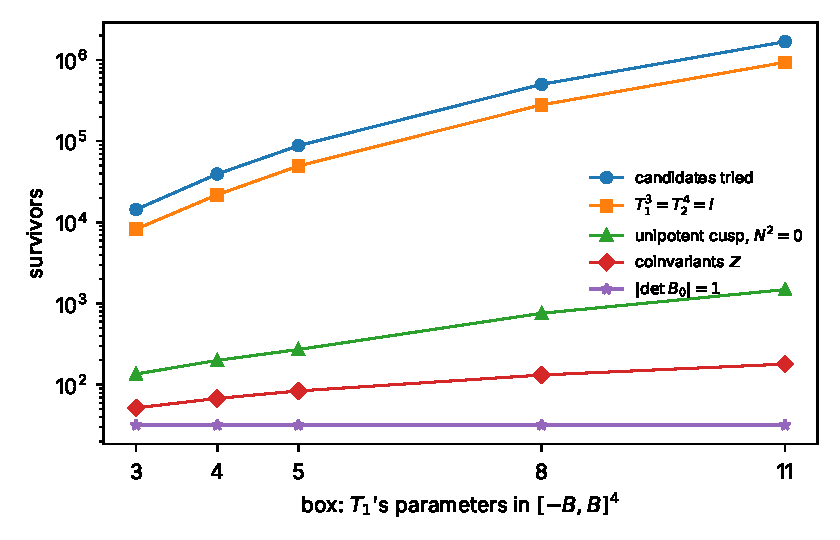
\includegraphics[width=0.62\textwidth]{sixsphere_funnel.pdf}
\caption{The funnel's stage counts against the box. Every stage but the last
keeps growing; the last is \SSUnimod{} throughout.}
\label{fig:funnel}
\end{figure}

\begin{observation}
\label{obs:stable}
At the boxes $\SSStabBoxes$ the final count is \SSStabFinal{}, while the
cusp stage grows \SSStabCusp{} (\cref{fig:funnel}). The condition
$|\det B_0| = 1$ appears to cut the infinite families to a finite set. We
have no proof. Separately, the closure stage has never removed a candidate,
which suggests it follows from the coinvariant condition in the flag class;
that too is unproved.
\end{observation}

\subsection{The classes}

\begin{proposition}
\label{prop:classes}
The \SSUnimod{} survivors form \SSClassesWord{} $\GL_4(\ZZ)$-conjugacy
classes of \SSClassSize{}. Exactly one class can reach $|p| = 1$.
\end{proposition}

\begin{proof}
Membership: for each survivor, the conjugating matrix is found by solving
the linear system $P T_j = T'_j P$ exactly and searching its integer points;
each is verified. Distinctness: the set of values of $|p|$, taken modulo
$m_1m_2 = 12$ as $\min(x, 12 - x)$, that admissible twists can reach is a
conjugacy invariant --- the functional $\gamma$ that reads off $\ell_j$ is
canonical up to sign --- and it takes a different value on each class:
$\SSGoodInvariant$ on one, and \SSOtherInvariants{} on the others. Only the
first contains $1$.
\end{proof}

The proof of distinctness does not depend on the conjugator search, which
could in principle miss a large conjugator: two classes with different
invariants cannot be conjugate, however hard one looks (\cref{fig:classes}). 

\begin{figure}[htbp]
\centering
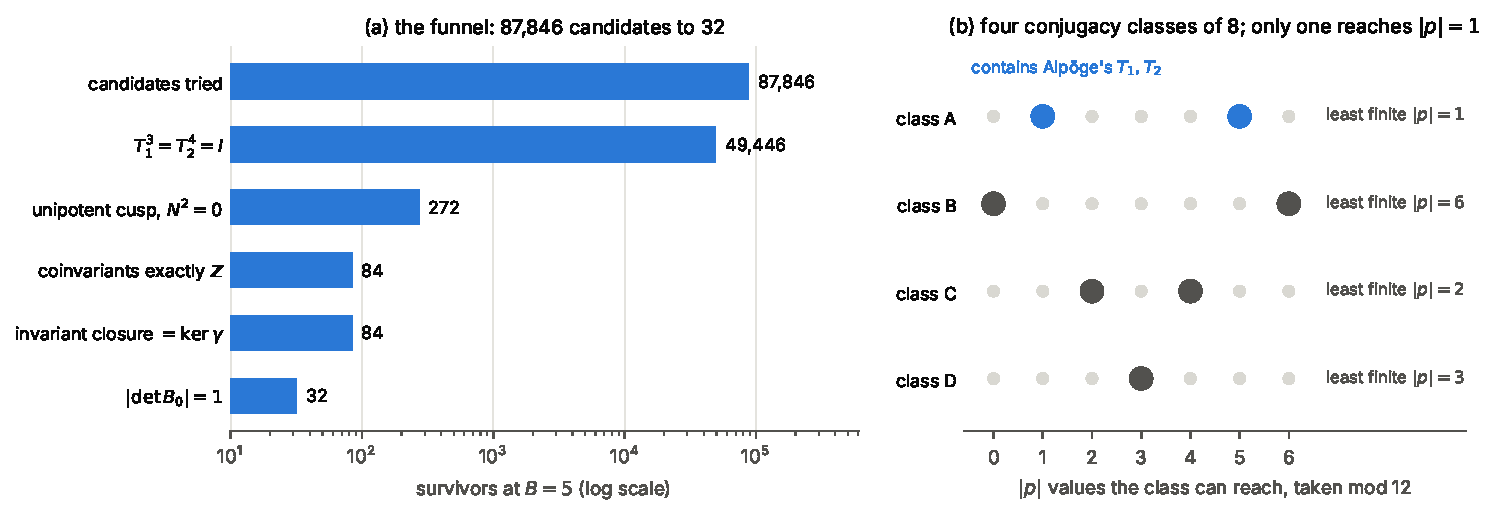
\includegraphics[width=\textwidth]{ss_funnel_classes.pdf}
\caption{(a) The funnel at $B = \SSBox$, on a log scale: the stage counts of the
table above, from \SSTried{} candidates to \SSUnimod{}. (b) The \SSUnimod{}
survivors form four $\GL_4(\ZZ)$-conjugacy classes of \SSClassSize{}. Each is
marked by the values of $|p|$, taken as $\min(x, 12 - x)$, that its admissible
twists can reach; the four sets partition $\{0, \dots, 6\}$, and only the class
containing Alpöge's matrices reaches $1$.}
\label{fig:classes}
\end{figure}

The class that reaches $|p| = 1$ is the paper's:

\begin{proposition}
\label{prop:paper}
The integer matrix
\[
  P = \SSPaperConj, \qquad \det P = \SSPaperConjDet,
\]
conjugates Alpöge's $(T_1, T_2)$ onto the normal-form representative of
the class that reaches $|p| = 1$.
\end{proposition}

This is checked by multiplication, and in Lean (\texttt{paper\_conjugator},
by \texttt{decide}). The other three classes bottom out at $|p| =
\SSNearMissMins$ respectively. Whether any of them supports the period
functions of the construction --- and so a compact complex threefold at all,
a rational homology sphere in the cases $|p| = 2, 3$ --- is a question about
the analytic side that we do not address.

% =====================================================================

\section{Results: the cusp fibre is the monotile's substrate}
\label{sec:laves}

\subsection{The substrate at the Hat point}

Every tile of the monotile family of Smith, Myers, Kaplan and
Goodman-Strauss~\cite{SmithHat,SmithSpectre} is a union of eight kites (\cref{fig:hat}) whose
two bond
lengths are the family's parameters: $a$ from hexagon centre to edge
midpoint and $b$ from edge midpoint to hexagon vertex, meeting at right
angles along directions that are multiples of $30^\circ$~\cite{SuppMonotile}.
Coordinates lie in $\QQ(\sqrt3)$ and are exact. At generic proportions a
hexagon's twelve outer kite corners stay distinct; at $a : b = \sqrt3 : 1$,
the Hat's proportions, and only there, they merge in pairs into the six
vertices of the $[3.4.6.4]$ Laves tiling~\cite{SuppMonotile}. The monotile
paper put it as: the substrate detects the Hat.

\begin{figure}[htbp]
\centering
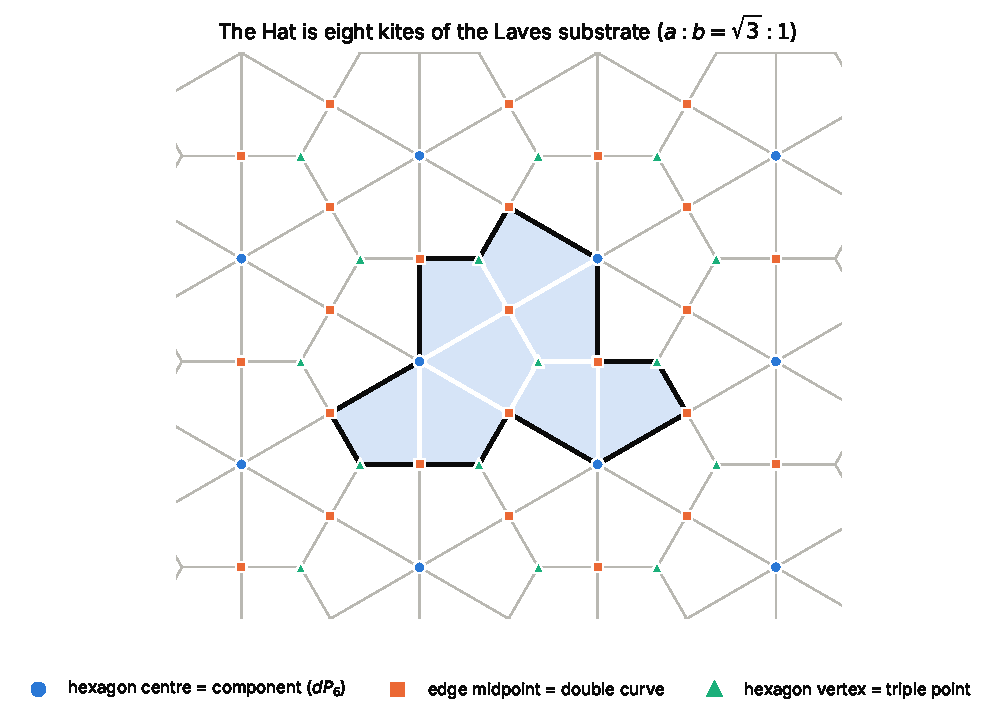
\includegraphics[width=0.78\textwidth]{ss_hat_kites.pdf}
\caption{The Hat at $a : b = \sqrt3 : 1$ as a union of eight kites of the
$[3.4.6.4]$ Laves lattice. Circles are hexagon centres (valence 6), squares
edge midpoints (valence 4), triangles hexagon vertices (valence 3). The heavy
outline is the Hat's thirteen-sided boundary; the eight kites inside it are
whole kites of the lattice, and their areas add to the Hat's, $8\sqrt3$ in
units where the shorter bond is $1$.}
\label{fig:hat}
\end{figure}

On the six-sphere's side, the cusp fibre is built from a toric fan whose
cross-section is the $A_2$ triangulation of the plane~\cite{Alpoge}: its
vertices give the components of $W$, its edges the double curves, its
triangles the triple points, and the quotient by $B_0\ZZ^2$ identifies them
(\cite[Part~III]{Impl}).

\begin{theorem}
\label{thm:laves}
At the Hat point $a : b = \sqrt3 : 1$, the monotile substrate is the Hasse
diagram of the $A_2$ triangulation: its sites are the cells --- hexagon
centres the vertices, edge midpoints the edges, hexagon vertices the
triangles --- and its bonds are exactly the cover relations vertex $<$ edge
$<$ triangle. At any other proportions it is not.
\end{theorem}

\begin{proof}[Computation]
Embed $A_2$ in the plane by $e_1 \mapsto 2a(\cos 30^\circ, \sin 30^\circ)$,
$e_2 \mapsto 2a(0,1)$, placing vertices at hexagon centres; edge midpoints
and triangle centroids follow (\cref{fig:dictionary}). For the two-ring patch of~\cite{SuppMonotile}
at the Hat point, all \SSLavesSites{} sites coincide exactly, in
$\QQ(\sqrt3)$, with cells of the matching kind, and the \SSLavesIncidences{}
cover relations among them are exactly its \SSLavesBonds{} bonds. At the
Spectre's proportions $a = b$, and at $17/10 : 1$ within $2\%$ of $\sqrt3$,
the corners do not merge: the patch has \SSSpectreSites{} sites and
\SSNearHatSites{} sites, its ``vertex'' sites have valence
\SSSpectreVertexValence{} rather than $3$, and the graph is a different
graph --- not a metric distortion of the same one. That the corners merge
at no other ratio is the exact coincidence computed in~\cite{SuppMonotile};
the two cases here exhibit the failure. Finally, the patch is finite but the
substrate is periodic, and the patch contains a fundamental domain together
with every cell incident to it, so the identity on the patch is the identity
everywhere.
\end{proof}

\begin{figure}[htbp]
\centering
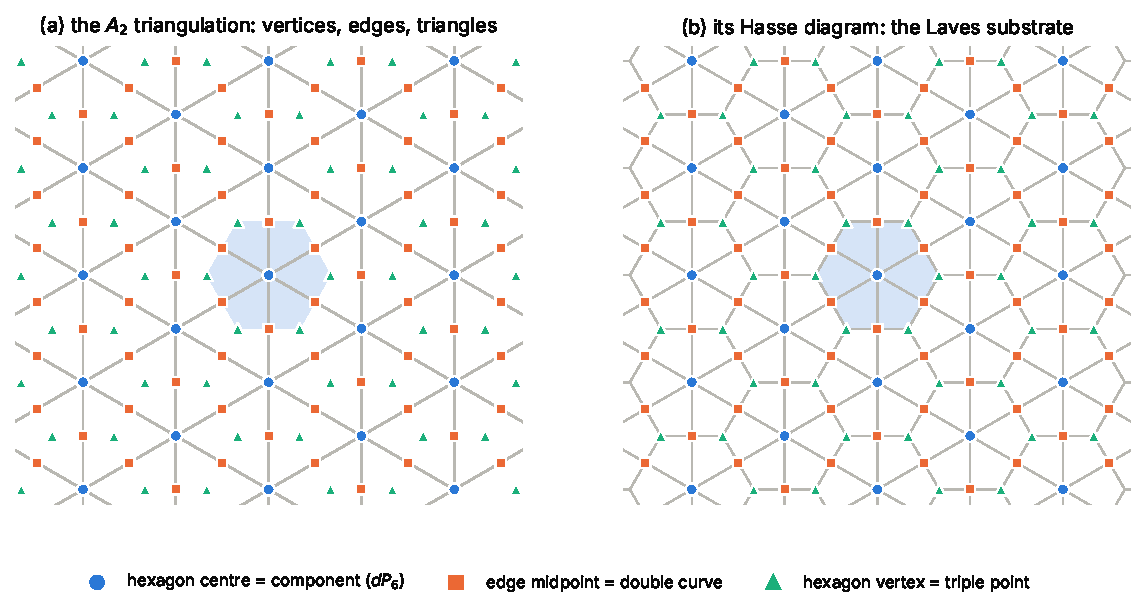
\includegraphics[width=\textwidth]{ss_dictionary.pdf}
\caption{\Cref{thm:laves} at the Hat point. (a) The cells of the $A_2$
triangulation, embedded as in the proof: vertices (circles), edge midpoints
(squares) and triangle centroids (triangles). (b) The Laves substrate on the
same sites; its bonds are exactly the cover relations vertex $<$ edge $<$
triangle. The shaded hexagon marks one hexagon centre with its six edge
midpoints and six hexagon vertices.}
\label{fig:dictionary}
\end{figure}

\begin{figure}[t]
\centering
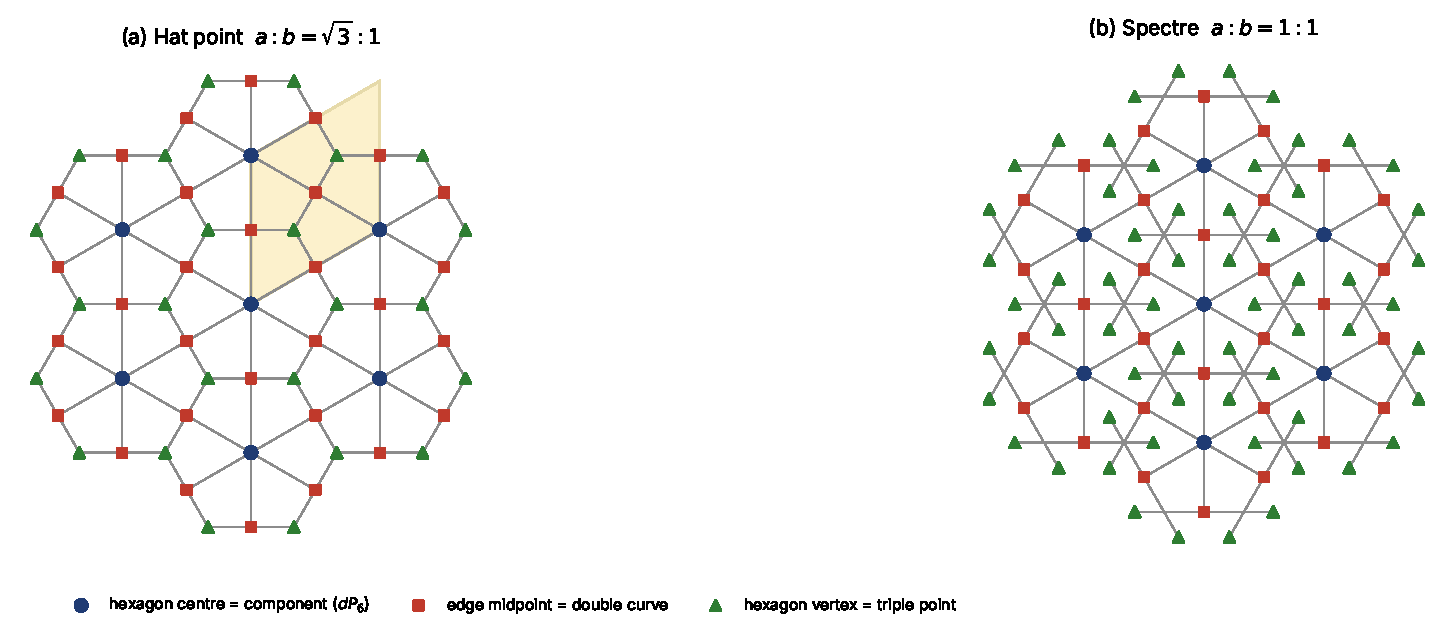
\includegraphics[width=\textwidth]{sixsphere_laves.pdf}
\caption{(a) The monotile substrate at the Hat point, with its sites marked by
the stratum of $W$ they become. The shaded parallelogram is one fundamental
domain of $B_0\ZZ^2$: it contains one hexagon centre, three edge midpoints and
two hexagon vertices, counted with the usual fractions --- one component,
three double curves, two triple points. (b) The same patch at the Spectre's
proportions: the outer corners stay paired and apart, and the graph is no
longer the Hasse diagram of anything.}
\label{fig:laves}
\end{figure}

\subsection{The dictionary}

Since $|\det B_0| = 1$, the translations by $B_0\ZZ^2$ are exactly the
translations of the Laves tiling by its period lattice, and the cusp fibre
is that tiling rolled up on $\RR^2 / B_0\ZZ^2$
(\cref{fig:torus,fig:dp6}):

\begin{center}
\small
\begin{tabular}{lll}
\toprule
Laves tiling at the Hat point & cusp fibre $W$ & per domain \\
\midrule
hexagon centre (valence 6) & a $dP_6$ component & \SSWComponents \\
edge midpoint (valence 4) & a double curve & \SSWCurves \\
hexagon vertex (valence 3) & a triple point & \SSWPoints \\
kite & a corner of the $dP_6$ hexagon & $6$ \\
centre--edge bond & a $(-1)$-curve of the hexagon & $6$ \\
edge--vertex bond & a double curve through a triple point & $6$ \\
\bottomrule
\end{tabular}
\end{center}

Three statements about $W$ proved in~\cite{Alpoge} and computed
in~\cite{Impl} now read as statements about the tiling:
\begin{itemize}[nosep]
\item $e(W) = \SSEW$: the torus orbits of $W$ have Euler characteristic
$0$ except the triple points, so $e(W)$ counts hexagon vertices in a
fundamental domain.
\item The rolled-up tiling is a torus: $6 - 12 + 6 = 0$ sites, bonds and
kites per domain.
\item Friedman's triple-point formula $(C|_V)^2 + (C|_{V'})^2 + T_C =
0$~\cite{Friedman}, which holds on every double curve of $W$, reads: each
edge midpoint is bonded to two hexagon vertices, and each hexagon side is a
$(-1)$-curve, so $-1 - 1 + 2 = 0$.
\end{itemize}

\begin{figure}[htbp]
\centering
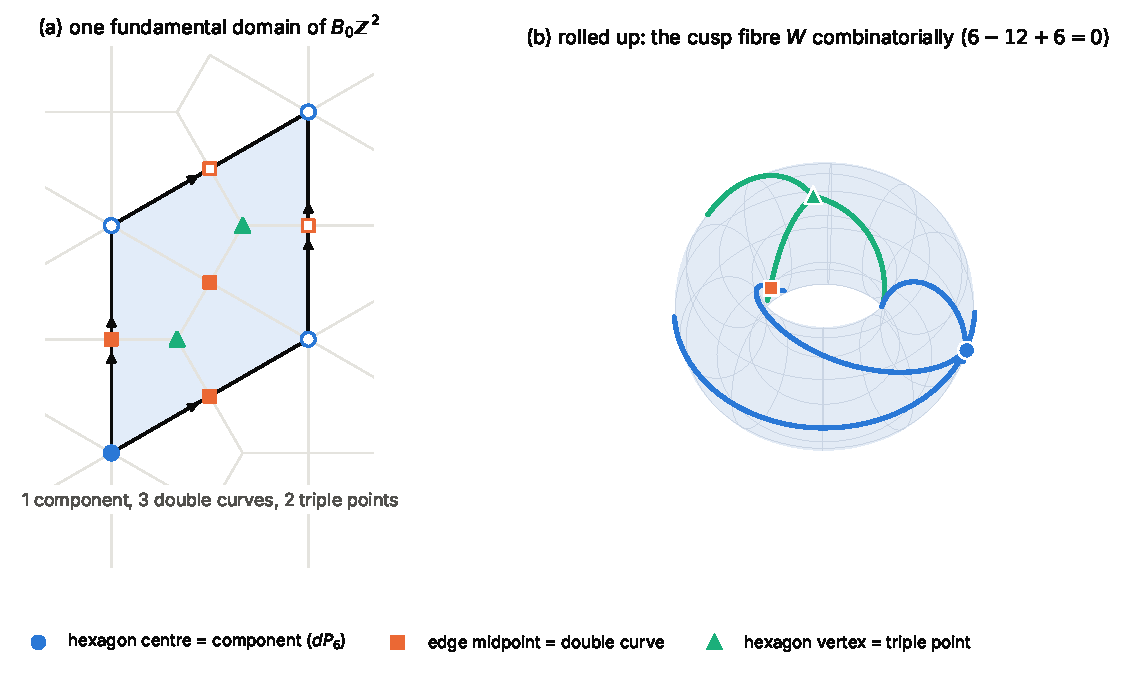
\includegraphics[width=\textwidth]{ss_torus.pdf}
\caption{(a) One fundamental domain of $B_0\ZZ^2$. Filled marks are its
representatives and hollow marks their images on the boundary; sides carrying
equal arrows are identified. It holds one component, three double curves and
two triple points. (b) The same sites and bonds on $\RR^2 / B_0\ZZ^2$, with
the far side of the torus hidden: $6 - 12 + 6 = 0$ sites, bonds and kites per
domain.}
\label{fig:torus}
\end{figure}

\begin{figure}[htbp]
\centering
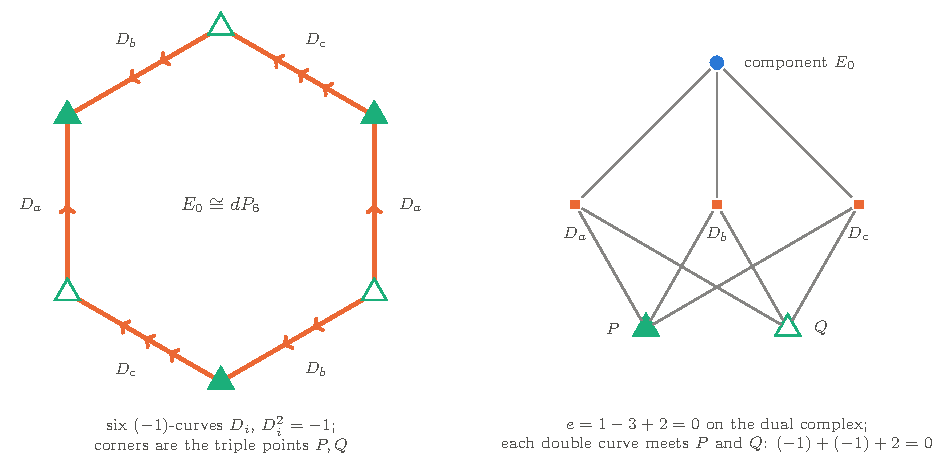
\includegraphics[width=\textwidth]{tikz_dp6_hexagon.pdf}
\caption{The component $E_0 \cong dP_6$ and the incidence structure of $W$.
Left: the hexagon of six $(-1)$-curves. Opposite sides are glued (equal arrow
counts) into the three double curves $D_a, D_b, D_c$, and the six corners
fall on two triple points, $P$ (filled) and $Q$ (hollow), alternating. Right:
the Hasse diagram of the strata, with $1$, $3$ and $2$ elements per rank; every
double curve passes through both triple points. Drawn from the data of
\texttt{sixsphere.cusp\_fibre}~\cite{Impl}.}
\label{fig:dp6}
\end{figure}

\subsection{What descends, and what does not}

The theorem is an identity of substrates, not of tilings, and the
distinction is the point. The Laves tiling is periodic, and its quotient by
$B_0\ZZ^2$ is a compact object --- the cusp fibre. A Hat tiling is
aperiodic: it is invariant under no translation lattice, $B_0\ZZ^2$
included, so it does not descend to $W$ or to any torus. In the language of
\cite{SuppMonotile}, whose subtitle is ``what has no momentum space'', the
cusp fibre is the same substrate equipped with exactly the momentum space
the monotile lacks. Both inherit their lattice from $A_2$, and the
six-sphere knows nothing about monotiles; what they share is that one
lattice, and --- by \cref{thm:laves} --- the single point of the monotile
family at which its substrate \emph{is} that lattice's incidence structure.

% =====================================================================

\section{Orientation Reversal and Lattice Duality}
\label{sec:mirror}

\begin{proposition}
\label{prop:achiral}
Reversing the orientation of the base replaces $(T_1, T_2)$ by
$(T_1^{-1}, T_2^{-1})$ \cite[Remark~3.18]{Alpoge}. The two pairs are
conjugate:
\[
  P = \SSMirrorConj, \qquad \det P = \SSMirrorDet,
\]
satisfies $P T_j P^{-1} = T_j^{-1}$ for $j = 1, 2$.
\end{proposition}

The monodromy therefore cannot distinguish $X$ from its orientation-reversed
counterpart. This is a statement about the lattice, not a proof that $X$ is
biholomorphic to its conjugate. It is machine-checked
(\texttt{lattice\_achiral}), and it fits the cross-domain framework
of~\cite{SuppFigures}, in which each domain has an involution and asks
which objects it fixes: here the involution is orientation reversal of the
base, it preserves the reachable $|p|$ residues $\{1, 5\}$ (as it must,
since $|p|$ is insensitive to sign), and the lattice data is a fixed point
--- in contrast with the Spectre, which is strictly chiral~\cite{SmithSpectre}.

\begin{proposition}
\label{prop:dual}
The monodromy lattice $V$ and its dual are isomorphic over $\QQ$ but not
over $\ZZ$: every integral intertwiner has determinant $\SSDualDetForm$ in
the coordinates $(s, t)$ of the rank-two lattice of intertwiners.
\end{proposition}

\begin{proof}
The invariant alternating form $Q_0$ of \cite[Lemma~2.8]{Alpoge} satisfies
$Q_0 T = T^{-t} Q_0$, so it intertwines $V$ and its dual over $\QQ$; but
$\det Q_0 = \SSDetQZero$. The intertwiners form a rank-two lattice, and the
determinant of the general one factors as $\SSDualDetForm$, which is never
$\pm 1$.
\end{proof}

\begin{sloppypar}
Alpöge shows the construction carries no polarization, because the form
$b(x, y) = Q_0(x, Ny)$ is indefinite. \Cref{prop:dual} is a sharper,
integral statement: there is not even a non-positive \emph{principal} one.
\end{sloppypar}

% =====================================================================

\section{Arithmetic Invariants and Resemblances to the Spectre}
\label{sec:arith}

The special values of the construction's period functions lie at the
elliptic points, $\tau(z_1) = e^{i\pi/3}$ and $\tau(z_2) = i$, generating
$\QQ(\sqrt{-3}, i) = \QQ(\zeta_{12})$. Its quadratic square classes are
$\SSClassesPeriods$ --- signed: dropping the sign, as an earlier helper in
the package did, would report the classes of the real field $\QQ(\sqrt3)$
and manufacture an identity with the monotile's geometry. With signs kept:

\begin{center}
\small
\begin{tabular}{lll}
\toprule
field & square classes & shared with $\QQ(\zeta_{12})$ \\
\midrule
six-sphere periods, $\QQ(\zeta_{12})$ & $\SSClassesPeriods$ & --- \\
monotile geometry, $\QQ(\sqrt3)$ & $\{1, 3\}$ & $\SSShareGeometry$ \\
Hat inflation, $\QQ(\sqrt5)$ & $\{1, 5\}$ & $\{1\}$ \\
Spectre inflation, $\QQ(\sqrt6, \sqrt{10})$ & $\SSClassesSpectre$ & $\{1\}$ \\
\bottomrule
\end{tabular}
\end{center}

The six-sphere shares the monotiles' \emph{geometry} field and none of their
\emph{inflation} fields --- consistent with \cref{sec:laves}, where it shares
the substrate and not the tiling.

Two further facts sharpen the picture. The Euclidean triangle groups are
$(2,3,6)$, $(2,4,4)$ and $(3,3,3)$; none contains both a $3$ and a $4$, so
the base orbifold of the construction is necessarily hyperbolic, while the
substrate's symmetry is the Euclidean $(2,3,6)$. And the cusp component's
polygon is the hexagon of the toric surface $B_3$, whose hopping vectors are
those of the triangular lattice: the mirror curve of the component is the
triangular-lattice Hofstadter model of~\cite{chen2025,shaffer2022, SuppMath}.

\paragraph{The $\sqrt6$.} The form $b = 6w^2 - \delta^2$ has isotropic
slopes $\pm\sqrt6$, and the Spectre's inflation factor is $\lambda =
(\sqrt6 + \sqrt{10})/2$, with $\lambda^2 = 4 + \sqrt{15}$: the two share the
square class $\SSShareLatticeSpectre$. The origins are unrelated. The
six-sphere's $6$ is $Q_0(u,w)$, forced by the entry $-6$ of $T_1$, which the
period laws pin down~\cite[Part~II]{Impl}; the Spectre's is a consequence of
its substitution matrix. Nothing downstream of either uses the other.

\paragraph{Valence four.} The Laves valences $(6, 4, 3)$ echo the orbifold
orders $(3, 4, \infty)$. But the valence-four sites are the double curves of
$W$, which lie over the cusp $p_0$ --- not over $p_2$, the point of order
four, whose fibre is a multiple fibre with no double curves at all.

% =====================================================================

\section{Connections to the Rest of the Package}
\label{sec:links}

The package this paper belongs to also computes, exactly, with polytopes,
with the lattice $H^2(K3,\ZZ)$ and with Bridgeland central charges on
Calabi--Yau threefolds. This section asks what the six-sphere's finite layer
shares with each. The computations are in \texttt{pyCICY.sixsphere\_links}
and are tested in \texttt{tests/test\_sixsphere\_links.py}; each number is
reached by at least two routes, and the constants are written by
\texttt{paper/make\_sixsphere\_facts.py}.

\subsection{The cusp component and the volume product}
\label{sec:links-mahler}

The component of the cusp fibre is the degree-six del Pezzo surface $dP_6$,
the toric surface whose polygon is $B_3$, the hexagon with \SSDPBoundary{}
boundary points. Its anticanonical degree $K^2$ is the normalised volume
$V(B_3) = 2\,\mathrm{Area}(B_3)$ (the identity $V(P) = (-K)^n$ for the
Gorenstein toric Fano variety whose anticanonical polytope is the reflexive
polytope $P$; $B_3$ is self-dual, so there is no ambiguity about which of the
pair is meant).

\begin{proposition}
\label{prop:dp6}
$K^2_{dP_6} = \SSDPKTwo$. This is computed four ways, with no shared code:
by triangulating the hexagon ($V(B_3) = \SSDPVolume$); by Ehrhart counts of
the same polygon; by Noether's formula $K^2 = 12 - n = 12 - \SSDPRays$ for a
smooth complete toric surface with $n$ rays~\cite{Fulton}; and as $9 - 3$ for
$\mathbb{P}^2$ blown up at three points. The toric divisors have
self-intersections $(-1)^{\times 6}$, summing to $12 - 3n = -6$ as they
must.
\end{proposition}

The hexagon is self-dual: $V(B_3^*) = \SSDPDual$, so the volume product is
$V(B_3)V(B_3^*) = \SSDPProduct$. It is centrally symmetric, and the Mahler
bound for symmetric bodies is $4^2\cdot 2! = \SSDPBoundSym$, so $B_3$ lies
strictly above it (only two reflexive polygons attain it). The number that
the dictionary of \cref{sec:laves} reads off as six kites per domain, six
$(-1)$-curves of the hexagon, six corners, is therefore also the volume of
the polytope; the agreement is the toric fact that a smooth toric surface has
as many torus-fixed points as rays, together with $K^2 = 12 - n$, and it is
specific to $n = 6$. We claim nothing beyond that.

\subsection{The elliptic fibration and the lattice module}
\label{sec:links-lattice}

The middle block of the monodromy is that of an elliptic family over
$\mathbb{P}^1$ with singular fibres over the three points of the orbifold,
so each local monodromy fixes a Kodaira type up to the usual inversion: order
$3$ means $\mathrm{IV}$ or $\mathrm{IV}^*$, order $4$ means $\mathrm{III}$ or
$\mathrm{III}^*$, and the cusp, being unipotent, is of type
$\mathrm{I}_n$ ($n = 1$ here). The Euler numbers of the singular fibres of an elliptic
surface over $\mathbb{P}^1$ sum to $12\,\chi(\mathcal{O})$.

\begin{proposition}
\label{prop:kodaira}
For orders $(3,4)$ and an $\mathrm{I}_1$ cusp there are \SSKodairaCandidates{}
candidate triples, with Euler totals $\SSKodairaTotals$. Exactly one is a
multiple of $12$:
\[
  \SSKodairaTriple, \qquad 8 + 3 + 1 = 12 .
\]
Its Jacobian is a rational elliptic surface; a K3 (total $24$) is impossible.
\end{proposition}

The same enumeration reproduces the two examples of \cref{sec:triangle},
$\mathrm{IV}^*+\mathrm{II}+\mathrm{I}_2$ for $(3,6)$ and
$\mathrm{III}^*+\mathrm{II}+\mathrm{I}_1$ for $(4,6)$, and so is checked
against the paper's own Euler arithmetic before being used for $(3,4)$. The
trivial lattice of such a surface is $U \oplus R$ with $R$ the root lattice
of the reducible fibres, and the Mordell--Weil rank is
$10 - 2 - \operatorname{rk}R$.

\begin{proposition}
\label{prop:roots}
The root lattices $E_6 \oplus A_1$ and $E_7$ embed in $E_8$ both integrally
and over $\QQ$. Integrally: the $\SSERootsEight$ roots of $E_8$ are generated
from its Cartan matrix; the roots orthogonal to one root $\alpha$ form $E_7$
($\SSERootsSeven$ roots, rank $7$, discriminant \SSEDiscSeven{}); those
orthogonal to an $A_2 \ni \alpha$ form $E_6$ ($\SSERootsSix$ roots, rank
$6$, discriminant \SSEDiscSix{}), and $A_1 = \langle \alpha \rangle \subset
A_2$ is orthogonal to it, giving $E_6 \oplus A_1$ of discriminant
\SSEDiscSixA{}. Over $\QQ$ the Hasse--Minkowski test of
\texttt{pyCICY.k3lattice} accepts both. A control fails as it should:
$E_7 \oplus \langle 3 \rangle$ has the right rank but the wrong
discriminant and does not embed. In all three configurations ($\mathrm{IV}^*
+ \mathrm{III} + \mathrm{I}_1$, $\mathrm{IV}^* + \mathrm{II} + \mathrm{I}_2$,
$\mathrm{III}^* + \mathrm{II} + \mathrm{I}_1$) the Mordell--Weil rank is
$\SSMWRank$.
\end{proposition}

So the paper's $(3,4,\infty)$ data and its $(3,6,\infty)$ example have the
same root part, $E_6 \oplus A_1$, although the fibres differ. The scope is
narrow. Euler counting shows that the local data is consistent with a
rational elliptic surface of that configuration; it does not show that the
six-sphere's family \emph{is} such a surface, and whether the configuration
exists is a question about the Miranda--Persson classification~\cite{MP86}
that we do not decide. The $\QQ$-embedding is a necessary condition only;
the integral statement is the explicit construction inside $E_8$.

\subsection{Where the central-charge module stops}
\label{sec:links-cc}

The central-charge module computes the charges $Z(E) = -\int e^{-B-i\omega}
\mathrm{ch}(E)$ (ordinary and square-root-Todd) of the large-volume
stability conditions announced for smooth projective threefolds with trivial
canonical bundle. They need a real class $\omega$ with $\omega^3 > 0$. The
six-sphere has $H^2(X,\mathbb{R}) = 0$, so it carries no such class: it is
not K\"ahler, and the module's own guard \SSGuardRefused{} the empty class. We record this as a result rather than a gap. The
finite layer behind the six-sphere is rigid, but the charges that give the
CICY side its stability-theoretic content have no counterpart here.

% =====================================================================

\section{Conclusion}
\label{sec:conclusion}

Two questions were asked of the lattice data behind Alpöge's complex
six-sphere. Was it forced? Within the flag class: the triangle group, yes,
by proof; the matrices, up to conjugacy, yes in every range searched, with
the finiteness of the search space the one step left unproved. What is it
connected to? Its cusp fibre is the aperiodic monotile's substrate, at the
monotile's own distinguished point, rolled up on a torus --- the one object
the monotile, by aperiodicity, can never be. Along the way the lattice
turns out achiral and not self-dual over $\ZZ$, its arithmetic meets the
monotiles' in their geometry and not in their inflation, and two
resemblances with the Spectre are coincidences.

None of this bears on whether the construction is correct; that rests on
analysis and topology and on the external formalization~\cite{Alexeev}.
What it shows is that the finite layer the construction stands on is rigid,
and that its rigid core is a familiar object.

The cusp fibre provides the exact algebraic scaffolding --- a periodic
substrate with a momentum space --- that the aperiodic Hat tiling lacks. The
six-sphere knows nothing of monotiles, and we draw no physical conclusion
from the contact: it is an identity of substrates, together with the
connections of \cref{sec:links}, which are identities of integers.

% =====================================================================

\newpage

\footnotesize

\section*{Declarations}

\subsection*{Funding}
The author received no specific funding for this work.

\subsection*{Competing Interests}
The author declares no competing interests.

\subsection*{Source code}
\label{sec:source}

The implementation is \texttt{pyCICY.sixsphere\_search.py} in the repository
at \url{https://github.com/brentharts/CICY}, with the verification suite
\texttt{tests/test\_sixsphere\_search.py}, the Lean facts in
\texttt{pyCICY.sixsphere\_lean.py}, and the connections of
\cref{sec:links} in \texttt{pyCICY.sixsphere\_links.py}
(\texttt{tests/test\_sixsphere\_links.py}), which use the polytope,
K3-lattice and central-charge modules.

\subsection*{Limitations} 
Everything in \cref{sec:triangle,sec:forced} is
restricted to the flag class; lattice data outside it is not searched.
\Cref{obs:sign,obs:stable} are finite searches. \Cref{thm:laves} is a
statement about substrates; it says nothing about monotile tilings beyond
the fact that they cannot descend. \Cref{sec:links}: the Kodaira
configuration and the lattice embeddings are consistency statements for the
local monodromy, not statements that the six-sphere's fibration is that
elliptic surface, and the rational embedding is a necessary condition only.
Every analytic question --- whether the
near-miss classes support a complex structure, whether $X$ is biholomorphic
to its conjugate --- is declined, as is the diffeomorphism $X \cong S^6$
itself.


\begin{thebibliography}{99}

\bibitem{Hopf48}
H.~Hopf,
\emph{Zur Topologie der komplexen Mannigfaltigkeiten},
in: Studies and Essays Presented to R.~Courant, Interscience, New York
(1948), 167--185.

\bibitem{Alpoge}
L.~Alpöge,
\emph{A compact complex threefold fibred by tori over the projective line,
and the six-sphere},
preprint (2026), \url{https://alpo.ge/s6.pdf}.

\bibitem{Engel}
P.~Engel,
pedagogical account of Alpöge's construction, expository notes (2026),
\url{https://philip-engel.github.io/S6.pdf}.

\bibitem{Alexeev}
B.~Alexeev,
\emph{Lean formalisation of the solution to the Hopf problem} (2026),
\url{https://github.com/plby/HopfProblem}.

\bibitem{CDP20}
F.~Campana, J.-P.~Demailly and T.~Peternell,
\emph{The algebraic dimension of compact complex threefolds with vanishing
second Betti number}, Compositio Math.\ \textbf{112} (1998), 77--91;
\emph{Corrigendum}, Compositio Math.\ \textbf{156} (2020), 679--696.

\bibitem{Friedman}
R.~Friedman,
\emph{Global smoothings of varieties with normal crossings},
Ann.\ of Math.\ \textbf{118} (1983), 75--114.

\bibitem{SmithHat}
D.~Smith, J.~S.~Myers, C.~S.~Kaplan and C.~Goodman-Strauss,
\emph{An aperiodic monotile},
Combinatorial Theory \textbf{4} (2024) 6,
\href{https://arxiv.org/abs/2303.10798}{arXiv:2303.10798}.

\bibitem{SmithSpectre}
D.~Smith, J.~S.~Myers, C.~S.~Kaplan and C.~Goodman-Strauss,
\emph{A chiral aperiodic monotile},
Combinatorial Theory \textbf{4} (2024) 13,
\href{https://arxiv.org/abs/2305.17743}{arXiv:2305.17743}.

\bibitem{Impl}
B.S.~Hartshorn,
\emph{What two integer matrices determine, and what only a proof can say:
exact methods for Alpöge's complex structure on the six-sphere},
\texttt{AlpogeSixSphere.md} in
\url{https://github.com/brentharts/CICY} (2026).

\bibitem{SuppMonotile}
B.S.~Hartshorn,
\emph{What Real-Space Geometry Determines, and What Has No Momentum Space:
Exact Methods for the Aperiodic Monotile Family},
Pre-print (2026), \url{https://doi.org/10.5281/zenodo.21893694}.

\bibitem{chen2025}
F.~Chen, W.~O.~Wang, J.~-X.~Zhang, L.~Balents, and D.~N.~Sheng. (2025). 
\emph{Topological Chiral Superconductivity in the Triangular-Lattice Hofstadter-Hubbard Model}. arXiv.
\url{https://doi.org/10.48550/arxiv.2509.02757}

\bibitem{shaffer2022}
D.~Shaffer, J.~Wang, L. H.~Santos (2022). 
\emph{Unconventional self-similar Hofstadter superconductivity from repulsive interactions.}
Nature Communications, 13. 
\url{https://doi.org/10.1038/s41467-022-35316-z}

\bibitem{SuppMath}
B.S.~Hartshorn,
\emph{What a configuration matrix determines, and what it does not: exact
methods for heterotic compactifications on CICYs},
Pre-print (2026), \url{https://doi.org/10.5281/zenodo.21844007}.

\bibitem{SuppFigures}
B.S.~Hartshorn,
\emph{Supplementary material: figures for the pyCICY-X package},
companion document (Pre-print 2026),
\url{https://doi.org/10.5281/zenodo.21843383}.

\bibitem{Fulton}
W.~Fulton,
\emph{Introduction to Toric Varieties},
Annals of Mathematics Studies \textbf{131}, Princeton University Press (1993).

\bibitem{MP86}
R.~Miranda and U.~Persson,
\emph{On extremal rational elliptic surfaces},
Math.\ Z.\ \textbf{193} (1986), 537--558.

\bibitem{graf2020}
P.~Graf and M.~Schwald (2020). 
\emph{On the Kodaira problem for uniruled Kähler spaces.}
Arkiv för Matematik, 58(2), 267–284. 
\url{https://doi.org/10.4310/arkiv.2020.v58.n2.a3}

\end{thebibliography}

\end{document}
